%%%%%%%%%%%%%%%%%%%%%%%%%%%%%%%%%%%%%%%%%%%%%%%%%%%%%%%%%%%%%%%%%%%%%%
% Original Source: Dave Richeson (divisbyzero.com), Dickinson College
% Modified By: Chen Yiyang
% 
% A one-size-fits-all LaTeX cheat sheet. Kept to two pages, so it 
% can be printed (double-sided) on one piece of paper
% 
% Feel free to distribute this example, but please keep the referral
% to divisbyzero.com
% 
% Guidance on the use of the Overleaf logos can be found here:
% https://www.overleaf.com/for/partners/logos 
%%%%%%%%%%%%%%%%%%%%%%%%%%%%%%%%%%%%%%%%%%%%%%%%%%%%%%%%%%%%%%%%%%%%%%

\documentclass[10pt,landscape,letterpaper]{article}
\usepackage{amssymb}
\usepackage{amsmath}
\usepackage{amsthm}
\usepackage{physics} % for vectors
%\usepackage{fonts}
\usepackage{multicol,multirow}
\usepackage{spverbatim}
\usepackage{graphicx}
\usepackage{ifthen}
\usepackage[landscape]{geometry}
\usepackage[colorlinks=true,urlcolor=olgreen]{hyperref}
\usepackage{booktabs}
\usepackage{fontspec}
\setmainfont[Ligatures=TeX]{TeX Gyre Pagella}
\setsansfont{Fira Sans}
\setmonofont{Inconsolata}
\usepackage{unicode-math}
\setmathfont{TeX Gyre Pagella Math}
\usepackage{microtype}

\usepackage{empheq}

% new:
\def\MT@is@uni@comp#1\iffontchar#2\else#3\fi\relax{%
  \ifx\\#2\\\else\edef\MT@char{\iffontchar#2\fi}\fi
}
\makeatother

\ifthenelse{\lengthtest { \paperwidth = 11in}}
    { \geometry{margin=0.4in} }
	{\ifthenelse{ \lengthtest{ \paperwidth = 297mm}}
		{\geometry{top=1cm,left=1cm,right=1cm,bottom=1cm} }
		{\geometry{top=1cm,left=1cm,right=1cm,bottom=1cm} }
	}
\pagestyle{empty}
\makeatletter
\renewcommand{\section}{\@startsection{section}{1}{0mm}%
                                {-1ex plus -.5ex minus -.2ex}%
                                {0.5ex plus .2ex}%x
                                {\sffamily\large}}
\renewcommand{\subsection}{\@startsection{subsection}{2}{0mm}%
                                {-1explus -.5ex minus -.2ex}%
                                {0.5ex plus .2ex}%
                                {\sffamily\normalsize\itshape}}
\renewcommand{\subsubsection}{\@startsection{subsubsection}{3}{0mm}%
                                {-1ex plus -.5ex minus -.2ex}%
                                {1ex plus .2ex}%
                                {\normalfont\small\itshape}}
\makeatother
\setcounter{secnumdepth}{0}
\setlength{\parindent}{0pt}
\setlength{\parskip}{0pt plus 0.5ex}
% -----------------------------------------------------------------------

\usepackage{academicons}

\begin{document}

\definecolor{mathBlue}{cmyk}{1,.72,0,.38}
\definecolor{defOrange}{cmyk}{0, 0.5, 1, 0.3}
\definecolor{codeInlineRed}{cmyk}{0, 0.9, 0.9, 0.45}

\everymath{\color{mathBlue}}
\everydisplay{\color{mathBlue}}

% for vector notation in this module
\newcommand{\vect}[1]{\boldsymbol{#1}}
\newcommand{\deff}[1]{\textcolor{defOrange}{\textbf{#1}}}
\newcommand{\codein}[1]{\textcolor{codeInlineRed}{\texttt{#1}}}
\newcommand{\citeqn}[1]{\underline{\textit{#1}}}

\footnotesize
%\raggedright

\graphicspath{ {./img/} }

\begin{center}
  {\huge\sffamily\bfseries CS2106 Cheatsheet (Midterm)} \huge\bfseries\\
  by Yiyang, AY21/22
\end{center}
\setlength{\premulticols}{0pt}
\setlength{\postmulticols}{0pt}
\setlength{\multicolsep}{1pt}
\setlength{\columnsep}{1.8em}
\begin{multicols}{3}


% -----------------------------------------------------------------------
\section{Operating System Introduction}
\subsection{OS Overview}
\subsubsection{Terminology}
\deff{Multi-Programming} - The ability of the OS to run multiple programs, of same of different users, simultaneously.
\\
\deff{Time-Sharing} - The ability of the OS to support multiple users to interact with machine using terminals. Need Multi-programming.

\subsubsection{Common OS Structures}
\deff{Monolithic} - OS is a big, special program. The traditional approach taken by most Unix variants.
\\
\textbf{Pros}: 1) Ability to follow good SE principles, 2) Better Performance
\\
\textbf{Cons}: Highly coupled components and complicated internal structures

\medskip

\deff{Microkernel} - OS consists of many minimal kernels each providing basic and essential facilities, and microkernels are linked via IPC.
\\
\textbf{Pros}: 1) Simplicity, 2) More robust and extensible, 3) Better isolation \& protection
\textbf{Cons}: Communication across components take time, which penalises performance

\medskip

Other structures: \deff{Layered Systems}, \deff{Client-Server Model}.



\subsection{Hypervisor}
\deff{Hypervisors} \textasciitilde \ monitors ("containers") for running virtual machines, which allows other OS to run and debug on it. There are 2 types of Hypervisors
\begin{itemize}
    \item \deff{Type 1 \textasciitilde} - an OS working directly on hardware. Typically faster but more complicated. Expensive to acquire.
    \item \deff{Type 2 \textasciitilde} - a software (but not an OS) running in host OS. Simpler and can be used to emulate hardware you do not have.
\end{itemize}




\section{Process Management}
\subsection{Process}
A \deff{Process} is an abstraction to describe a running program. A \deff{Process Control Block} (PCB) (aka. \deff{Process Table Entry}) is a unit entity storing necessary information (\deff{Execution Context}) for a process. The \deff{Process Table} stores all  current PCBs.
\\
Context for a \textbf{Context Switch} includes: 1) Registers (GPR \& Special), 2) Stack Pointer, and 3) PC.

\subsubsection{Generic 5-State Process Model}
The Generic 5 States are: \deff{New}, 2) \deff{Ready}, 3) \deff{Terminated}, 4) \deff{Running}, and 5) \deff{Blocked}.
\\
\underline{Note:} Some systems (including Unix) do not have New - whenever a process is created, it is in Ready.

\medskip

In addition, in Unix, there are \deff{Orphan Process}, which is a child process with parent terminated before it, so the orphan is "adopted" by \codein{init} and waited properly when done, and 2) \deff{Zombie Process}, which is a child that has exited but the parent is executing but does not call wait on the child.

\subsection{Memory Regions}
The Memory consists of 1) \deff{Text} for instructions, 2) \deff{Data} for global variables, \deff{Heap} for dynamic allocation, e.g. via \codein{malloc()} in C, and 4) \deff{Stack} for function invocations.


\subsection{Stack \& Function Calls}
\subsubsection{Terminology}
In a function call, \deff{Caller} function invokes a function call of \deff{Callee}.
\\
A \deff{Stack Frame} stores information about one callee invocation, and there are two associated pointers. \deff{Stack Pointer} (SP) points to the top of the Stack while \deff{Frame Pointer} (FP) points to a fixed location in a Stack Frame.
\\
\underline{Note:} FP facilitates easy access of Stack Frame items. It is platform dependent and not compulsory. Every platform has SP.
\\
\deff{Register Spilling} is the practice of using memory to temporarily store GPRs' values so that GPRs can used reused for other purposes and restored afterwards. It is used during callee invocation.
\\
In a function call, \deff{Stack Frame Setup} is the preparation to make a function call, and \deff{Stack Frame Teardown} is the returning from function call.

\subsubsection{Stack Frame Setup and Teardown Example}
In \deff{Frame Setup}, \underline{Caller:} 1) Pass parameters with registers and/or stack, and 2) Save Return PC on stack; \underline{Callee:} 1) Save old SP, 2) Allocate space for local variables on stack, and 3) Adjust SP to point to new stack top.

\medskip

In \deff{Frame Teardown}, \underline{Callee:} 1) Place return result on stack (if applicable), and 2) Restore saved SP; \underline{Caller:} 1) Utilise return result (if applicable), and 2) Continue execution in caller following return PC.


\subsection{System Calls}
\deff{System Call} (aka. \deff{Syscall}) \textasciitilde \ API to OS, and it changes from User Mode to Kernel Mode (and changes back to User Mode after the syscall has completed). There are 3 ways of using Syscalls.
\begin{enumerate}
    \item Use the library version of the syscall. The library version serves as a \textbf{function wrapper} and typically has the same name. Applicable to most syscalls in modern languages.
    \item Use the user-friendly library version of the syscall. This version has related handles and serves as a \textbf{function adapter}. Few syscalls have such.
    \item Use the language's syscall method directly. E.g. in C, \codein{long syscall(long number, ...)}.
    
\end{enumerate}



\subsection{Exceptions, Traps \& Interrupts}
\deff{Exception} - Executing a machine level instruction can cause exceptions, e.g. arithmetic errors or memory accessing errors, and exception handlers are executed. Exceptions are \textbf{Synchronous}. 

\medskip

\deff{Trap} - Exceptions intentionally set-up. Trap is an easy-to-use mechanism to enter kernel mode. Aka. "software interrupts".

\medskip

\deff{Interrupt} - External events can cause interrupts during the execution of a program, as a form of notification, and interrupt handlers are executed. Interrupts are usually hardware-related and \textbf{Asynchronous}.



\section{Process Scheduling}
\subsection{Scheduling Overview}
Scheduling requires \deff{Scheduler}, the CPU component for process scheduling and \deff{Scheduling Algorithm}, that determines which process gets scheduled first.
\\
Depending on whether a process spends majority of time on CPU computation or I/O activity, it can be categorised as \deff{CPU Bound} or \deff{I/O Bound} activity.

\subsubsection{Types of Environment}
\begin{itemize}
    \item \deff{Batch Processing} - No user interaction or need to be responsive. Typically use non-preemptive scheduler since easier to implement.
    \item \deff{Interactive} - Involve user interaction and need to be responsive. Typically preemptive.
    \item \deff{Real-time} - All tasks have strict deadlines to meet and tasks are usually periodic.
\end{itemize}

\subsubsection{Types of Scheduling Policies}
\begin{itemize}
    \item \deff{Non-preemptive} - aka cooperative. A process stays scheduled until it blocks or gives up CPU voluntarily.
    \item \deff{Preemptive} - CPU can be taken from running process at any time.
\end{itemize}

\subsubsection{Scheduling Criteria}
All scheduling policies consider 1a) Fairness, whether it is biases against / towards any process, 1b) whether all processes can run without \deff{Starvation}, 2) Balanced utilisation of system resources, 3) \deff{Throughout}, number of tasks finished per unit time, 4) \deff{Turnaround Time}, total clock time taken (which is related to total/average waiting time), and 5) \deff{CPU Utilisation}, \% of time when CPU is working.
\\
In addition, Interactive System scheduling policies consider: 1) \deff{Response Time}, time between request and response by system, and 2) \deff{Predictability}, as it aims for less variance in response time.


\subsection{Batch Processing Scheduling Policies}
\subsubsection{First-Come First-Serve(FCFS)}
Maintain a Queue and add to Queue when new processes come. Run a task until it finishes or blocks, then choose next in Queue to run.
\\
\underline{Analysis:} Non-preemptive. No starvation. Sub-optimal avg waiting time.


\subsubsection{Shortest Job First (SJF)}
Maintain a Priority Queue of tasks to be scheduled, sorted in ascending order by the \textbf{estimated} CPU time needed for each task. 
\\
\underline{Analysis:} Non-preemptive. Starvation possible. CPU time can be estimated from the processes' past running time.

\subsubsection{Shortest Remaining Time (SRT)}
Preemptive version of SJF, where a new task can preempt currently running task if the estimated time for the former is less than remaining time needed for the latter.
\\
\underline{Analysis:} Preemptive. Starvation possible. Provide good service for short jobs.


\subsection{Interactive System Scheduling}
\subsubsection{Overview}
\deff{Time interrupt} is an interrupt that goes off periodically based on hardware clock and its handler invokes the scheduler to preempt a task. \deff{Interval of Time Interrupt} (ITI) is the timer period, i.e. smallest unit time in hardware clock for the timer. \deff{Time Quantum} is the execution duration given to a process, which can be constant or variable. It must be multiples of ITI.


\subsubsection{Round Robin (RR)}
Preemptive version of FCFS, where it runs the current task either until it blocks or gives up CPU, or when the time slice (\deff{quantum}) elapses. In the latter situation, put back the task to the rear of Queue.
\\
\underline{Analysis:} Preemptive, with a timer interrupt required. Response time guarantee, no starvation. Choice of quantum length affects performance.

\subsubsection{Priority Scheduling}
Maintain a Priority Queue and assign a priority value to every task to be scheduled. Choose tasks with highest priority every time. It can be preemptive or non-preemptive depending on whether higher priority tasks can preempt currently running tasks.
\\
\underline{Analysis:} Low priority tasks can starvation and preemptiveness does not help.


\subsubsection{Multi-Level Feedback Queue(MLFQ)}
Maintain multiple FIFO Queues of different priorities. Always pick from Queues of higher priority first, and run RR within each Queue. When a new task comes, put it in the highest priority Queue. Every time the tasks fully utilises its time slice, reduce its priority, otherwise retain its priority.
\\
\underline{Analysis:} Adaptive, seeking to minimise both response and turnaround time. Starvation possible. High priority Queues tend to have shorter time slices. Yet, possible to exploit the policy.


\subsubsection{Lottery Scheduling}
Scheduling is done rounds, where in each round, tasks are assigned "lottery tickets", the number of which depends on tasks' priority / estimate time. When picking a process to schedule, pick a ticket randomly from the pool then remove the task's tickets from the pool and pick from remaining tasks next time, until all tasks scheduled once for this round. New processes are not allowed to participate halfway during a round.
\\
\underline{Analysis:} Response time guarantee and no starvation. Good level of control. Simple.


\section{Inter-Process Communication}
\subsection{Common Mechanisms}
\subsubsection{Shared Memory}
Create a shared memory region once, and attach processes to the shared memory. All processes attached can read and write in shared memory just like to normal variables, achieving \textbf{implicit communication}. When done, detach all processes from the region and destroy it.
\\
\underline{Pros:} 1) Efficient, as no OS involvement during read and write to shared region, and 2) Ease of Use, as the implementation is simple and can be used for data of any type and size.
\\
\underline{Cons:} 1) Limited to a single machine, and 2) Synchronisation required as race conditions for shared variables can happen.


\subsubsection{Message Passing}
\textbf{Explicit} communication through exchange of messages. Process 1 prepares a message and send it to OS and Process 2 can receive it later. Both sending and receiving are syscalls.
\\
\underline{Pros:} 1) Safe, as guarded by OS, 2) Applicable beyond a single machines, 3) No need to synchronise.
\\
\underline{Cons:} 1) Inefficient, as all steps involve OS, 2) Hard to use, as data need to be packed/unpacked to supported message format.

\medskip

There are different variants of Message Passing, depending on its Naming Scheme and Synchronisation Behaviours.
\\
\deff{Naming Scheme} \textasciitilde \ How the sender/receiver identify one another
\begin{itemize}
    \item \deff{Direct Communication} - Send/Receiver explicitly names the other party. A form of 1-to-1 linkage. \underline{Pros:} Simple. \underline{Cons:} Impractical, especially since it requires the Receiver to know who sends it a message.
    \item \deff{Indirect Communication} - Messages are sent to / read from message storage (aka. \deff{Mailbox}), which can be shared among multiple processes. \underline{Pros:} Ability to have multiple senders and receivers.
\end{itemize}

\deff{Synchronisation Behaviour} \textasciitilde \ whether sending/receiving message is blocked until it is received/has arrived. For this module, assume \textbf{all receiving is blocked}.
\begin{itemize}
    \item \deff{Asynchronous MP} - Non-blocking Send. \underline{Pros:} Better flow for sender. \underline{Cons:} 1) Too much freedom for programmer, and 2) Not true asynchronous as \textbf{buffer size is finite}, so sending will block when buffer full.
    \item \deff{Synchronous MP} - Blocking Send, aka Rendezvous.
\end{itemize}
Synchronous MP can also be used as a form of synchronisation of two processes by using dummy message.



\subsection{Unix-Specific Mechanisms}
\subsubsection{Pipes}
In Unix, a process has 3 default communication channels, 1) \codein{stdin} for std input, 2) \codein{stdout} for std output, and 3) \codein{stderr} for std error output.

\medskip

Unix pipes behave like anonymous files, FIFO for data accessing order. Writer wait when pipe buffer is full, and reader waits when buffer empty. This enables Pipe to have \textbf{asynchronous} and \textbf{implicit} synchronisation.
\\
In addition there are \deff{half-duplex} (unidirectional) and \deff{full-duplex} (bidirectional) pipes.

\subsubsection{Signals}
\deff{Signals} are \textbf{asynchronous} (meaning can be sent anytime) notifications regarding an event, sent to a process/thread. The recipient must handle the signal by 1) a default set of handlers, or 2) user supplied handlers. \underline{Note:} Not all signal handlers can be override by user.
\\
Signals are sent from OS to user programs or from one user program to another. Signal handlers run in User Mode.
\\
With user supplied signal handlers, signals can achieve IPC.





\section{Threading}
\subsection{Threading Overview}
One process can have multiple threads, thereby achieving \deff{Data Parallelism} (different threads same task different data) and \deff{Task Parallelism} (different threads different tasks).
\\
\underline{Pros:} 1) Economy, as multi-threading easier than multi-processing, 2) Resource sharing, 3) Responsiveness, of multi-threaded programs, and 4) Scalability, as multi-threaded programs can utilise multiple cores / CPUs.
\\
\underline{Cons:} 1) Synchronisation getting more complicated, 2) Difficulty with \deff{System Call Concurrency}, and 3) Concerns regarding process behaviours (e.g. fork a multi-threaded process). 

\medskip

Certain information are shared across threads of the same process and some not shared.
\\
\underline{Shared:} 1) Text (code), 2) Data, 3) Heap, 4) File, and 5) Process ID.
\\
\underline{Not Shared:} 1) Thread Id, 2) Stack, 3) Registers (GPR \& Special), 4) PC



\subsection{Thread Implementation}
\subsubsection{User Thread}
\deff{User Thread} \textasciitilde \ Implemented as a user library. Not "recognised" or scheduled by the OS.
\\
\underline{Pros:} 1) Multi-threading can be done on any systems, 2) Context switch of threads easier, and 3) more configurable and flexible.
\\
\underline{Cons:} Sub-optimal performance with OS scheduling only processes.

\subsubsection{Kernel Thread}
\deff{Kernel Thread} \textasciitilde \ Implemented in OS, with thread operations handled as syscalls. Kernel schedules threads not processes.
\\
\underline{Pros:} Kernel can schedule threads.
\\
\underline{Cons:} 1) Slower and more resource-intensive with thread operations as syscalls, and 2) Generally less flexible.

\subsubsection{Hybrid Thread}
\deff{Hybrid Thread} \textasciitilde \ OS schedules only kernel threads while user threads can bind to kernel threads. More flexible.

% Illustration!


\section{Synchronisation}
\subsection{Critical Section}
\deff{Race Condition} - Interleaving of accesses to a shared modifiable resource. Race condition may lead to incorrect program behaviour so it is handled using \deff{Critical Section} (CS), which is designated code segment with race conditions. At any point of time, at most one process can be in the critical section.

\medskip

Critical Section has 4 properties:
\begin{enumerate}
    \item \deff{Mutual Exclusion} - If Process $P_1$ is in CS, all other processes are prevented from entering CS.
    \item \deff{Progress} - If no process is in a CS, one of the waiting processes should be granted access.
    \item \deff{Bounded Wait} - After Process $P_1$ requests to enter CS, there exists an upper bound on number of times other processes can enter CS before $P_1$.
    \item \deff{Independence} - Processes not executing in CS should never block (those waiting to enter CS).
\end{enumerate}
\underline{Note:} \#2 Progress requires \#4 Independence first, but it is possible to have \#4 Independence without \#2 Progress.
\\
\underline{Note:} \#2 Progress ensures no \deff{Deadlock}, a situation where all processes are blocked, and no \deff{Livelock}, a situation where all tasks are running but they do not "make any progress".


\subsection{HLL Implementation}
High-level Language (HLL) Implementations for Synchronisation are those using only normal programming constructs. (Use your brain power LOL)


\subsubsection{Failed Attempts}
\textbf{Attempt 1 - Lock Variable}: Use a shared boolean, \codein{lock}, to indicate whether any process in CS currently. Busy-wait if \codein{lock == 1}. Enter and update it if \codein{lock == 0}.
\\
\underline{Analysis:} \textbf{NOT WORK} as there can be race condition on \codein{lock} as well, violating \# 1 Mutual Exclusion.

\medskip

\textbf{Attempt 2 - Disable Interrupt}: As a fix to Attempt 1, disable interrupt (and hence no context switching) before a process waits or enters CS, and re-enable interrupts after it leaves CS.
\\
\underline{Analysis:} \textbf{NOT RECOMMENDED} as it only works on single-core systems and there can be race conditions with processes running on other cores in multi-core systems. In addition, disabling interrupts requires permission and is dangerous.

\medskip

\textbf{Attempt 3 - Turn Variable}: Use a shared variable, \codein{turn}, to indicate which process' turn it is currently. A process checks turn variable and waits until it is its own turn to enter CS.
\\
\underline{Analysis:} \textbf{NOT WORK} as it may violate \#4 Independence (\codein{turn = 0} and $P_1$ busy-waits but $P_0$ never enters CS).

\medskip

\textbf{Attempt 4 - Want Variable}: Use a shared boolean array, \codein{want[]}, where each element \codein{want[i]} indicates if Process $P_i$ wants to enter. (In case of 2 processes,) enter if the other process does not want to enter, otherwise wait.
\\
\underline{Analysis:} \textbf{NOT WORK} as it can have a deadlock when \codein{want[0] == 1} and \codein{want[1] == 1}, thereby violating \#2 Progress.


\subsubsection{Synchronisation Algorithms}
\deff{Peterson's Algorithm} - Combine Attempt 3 and 4. (In case of 2 processes,) wait if the other is waiting and it is the other's turn. If it is my turn, I will enter regardless.
\\
\underline{Analysis:} \textbf{WORK}, but 1) difficult to generalise for $\geq 3$ processes, and 2) Busy waiting is used and it is not desired.


\subsection{Assembly Level Implementation}
\deff{Test-Set-Lock} (TSL) \textasciitilde \ Similar to HLL Attempt 1 Using Lock Variable, but TSL does not have race condition because it is an \deff{Atomic}, i.e. reading and writiing of the variable can only be done by one process at any time, operation ensured by the hardware.
\\
\underline{Cons:} Busy waiting.


\subsection{HLL Abstraction}
\subsection{Semaphore}
\deff{Semaphore} - A generalised synchronisation mechanism with functional behaviour of wait and signal. 

\subsubsection{Implementation}
\begin{itemize}
    \item An integer \codein{S} \textasciitilde \ number of "net wake-ups". Can be initialised to any non-negative integer.
    \item \codein{wait(S)} - decrement \codein{S}, and if $S \leq 0$, (process calling the semaphore) blocks. Aka. \codein{P()} or \codein{down()}.
    \item \codein{signal(S)} - increment \codein{S}, and wait up one sleeping process if any. Aka. \codein{V()} or \codein{up()}.
\end{itemize}
\underline{Note:} Assume no negative value for semaphore in this module.

\subsubsection{Functionality}
A \deff{Binary Semaphore} that \textbf{initialises to 0} and \textbf{ensures only value 0 or 1} is a \deff{Mutex}, i.e. Mutual Exclusion, for preventing race conditions.
\\
\underline{Note:} Deadlock can be avoided but is possible with improper implementation of two or more mutexes.

\medskip

A \deff{General Semaphore} serves as a General Synchronisation Tool (not CS in this case) for multiple processes (e.g. ensuring Processes $P_1, P_2, P_3$ operate in a fixed order.
\underline{Note:} Semaphore do not use busy waiting.


\subsection{Others}
\deff{Conditional Variable} - An implementation that allows a task to wait for certain event to happen. It can \deff{broadcast}, which wakes up all waiting tasks.


\noindent\rule{8cm}{0.4pt}



\section{Intermediate Results \& Summary}
\subsection{From Tutorials}
\citeqn{(Tut1 Qn7)} In \codein{int *a = (int *) malloc(sizeof(int));}, the data, \codein{*a}, is created in the Heap while the pointer to this data, \codein{a}, can be in Stack or Data.

\subsection{From Past Questions}
\citeqn{(AY15/16Sem1 Qn1)} Library calls are language dependent, while syscalls depend only on the OS.

\medskip

\citeqn{(AY17/18Sem1 Qn8)} In scheduling, \textbf{Short Response Time} is not the same as \textbf{Bounded Waiting Time}. RR ensures latter but not former.



\subsection{Diagrams}
Onion Model of an Operating System:
\\
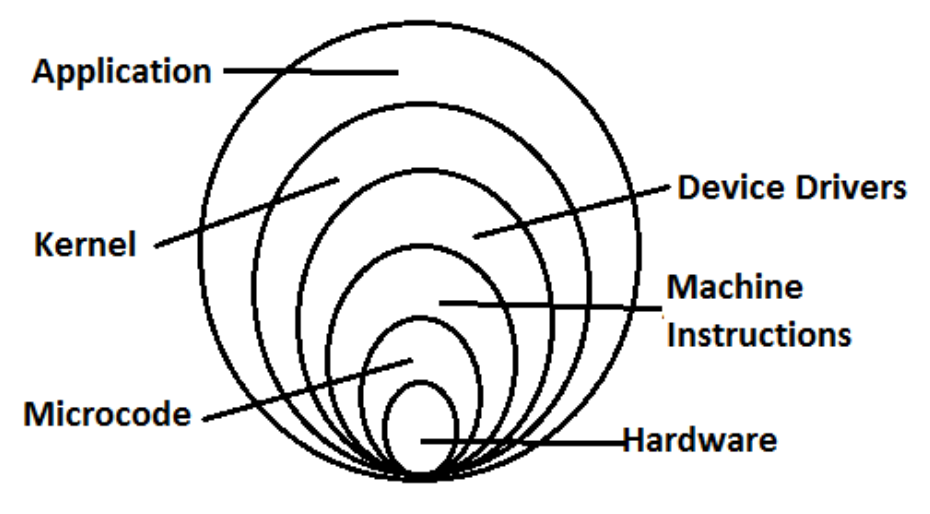
\includegraphics[width=8cm]{img/01_onion_model.png}

Generic 5 States of a Process:
\\
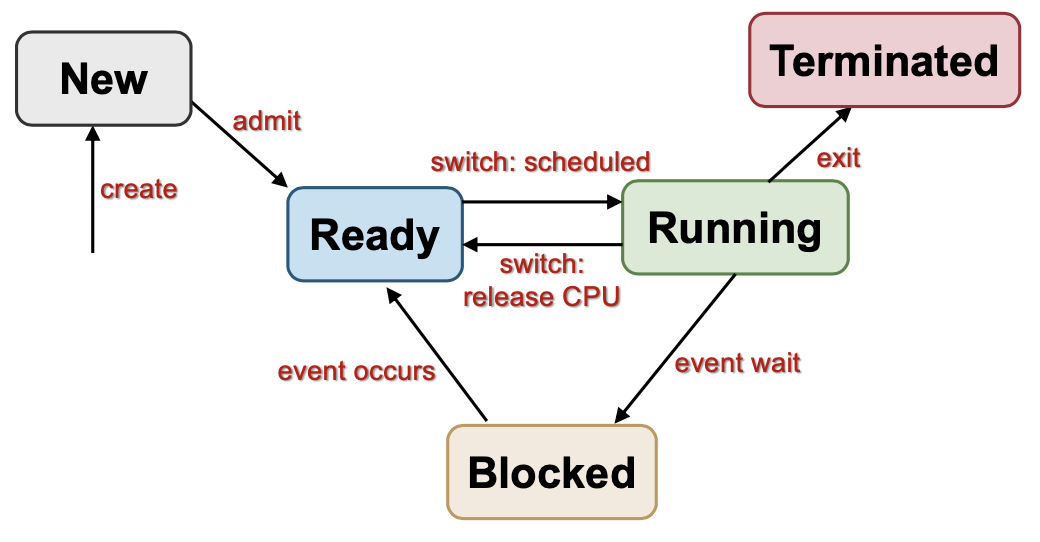
\includegraphics[width=8cm]{img/02_process_5_state.png}

Pseudocode for Peterson's Algorithm (note the order of updating variables before busy-wait):
\\
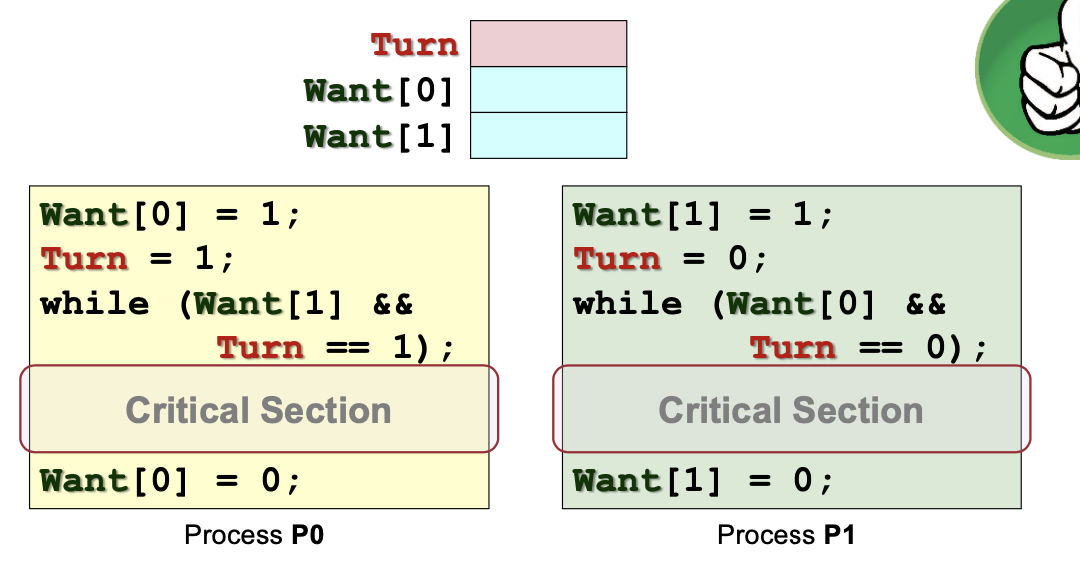
\includegraphics[width=8cm]{img/06_peterson.png}





\newpage




\section{Unix System Calls}
\subsection{Common Process Management Syscalls}
\subsubsection{\codein{fork()} Syscall}
\codein{int fork()} creates a duplicate of current process as a child process. It clones everything except PID and PPID. It returns the PID of child process forked in parent process and \codein{0} in child.
\\
Need header \codein{<unistd.h>}.


\subsubsection{\codein{exec*()} Family}
The family of syscalls, \codein{int exec*(...)}, replaces current executing process with a new one. It takes in path to the executable and arguments. It will not return when executing successfully and return \codein{-1} when fails.
\\
There are many variants, such as \codein{execv}, \codein{execl}, \codein{execle}, \codein{execlv}, or \codein{execv}, each with a slight difference in parameter specifications and behaviours.
\\
The typical usage is to create a new child process using \codein{fork()} then run the program using \codein{exec()} in the child.
\\
Need header \codein{<unistd.h>}.


\subsubsection{\codein{exit()} Syscall}
\codein{void exit(int status)} terminates the current process and the value of \codein{status} will return to the parent. The convention is \codein{0} for normal termination and non-zero for error.
\\
\codein{exit()} is the friendly wrapper of \codein{\_exit()} as the former does some necessary clean-up before invoking the syscall.
\\
When a child calls \codein{exit()}, it sends \codein{SIGCHLD} signal to the parent.
\\
Need header \codein{<unistd.h>}

\subsubsection{\codein{wait()} Family}
\codein{int wait(int *status)} makes the process block and wait for any one child process to terminate, and the exit status value is stored in the parent's variable referrenced by \codein{*status}. It cleans up remainder of terminated child's system resources.
\\
There are other variants such as \codein{waitpid()} that waits for a specific child.
\\
Need header \codein{<sys/types.h>} and \codein{<sys/wait.h>}.

\subsubsection{\codein{getpid()} Family}
\codein{int getpid()} returns the PID of the current process.
\\
There are similar syscalls such as \codein{getppid()}.
\\
Need header \codein{<unistd.h>}.



\subsection{IPC-Related Syscalls}
\subsubsection{\codein{pipe()} Syscall}
\codein{int pipe(int fd[2])} creates a unidirectional pipe channel with file descriptors \codein{fd[0]} for reading end and \codein{fd[1]} for writing end. It returns \codein{0} for successful creation and non-zero values for error.
\\
Need header \codein{<unistd.h>}.

\subsubsection{\codein{dup2()} Syscall}
\codein{int dup2(int oldfd, int newfd)} replaces the file descriptor of \codein{newfd} with the one specified by \codein{oldfd}.
\\
The syscall is typically used to redirect standard channels of a process to a pipe or file.
\\
Need header \codein{<unistd.h>}.



\subsubsection{Shared Memory Syscalls}
\codein{shmget()}, \codein{shmat()}, \codein{shmdt()}, and \codein{shmctl()} are syscalls to 1) create a shared memory region, 2) attach the shared memory to the current process, 3) detach the shared memory from the current process, and 4) destroy the shared memory region respective.
\\
\underline{Note:} \codein{shmget()} returns the ID of the shared memory created, and the ID is the identifier for the shared memory. A memory address is generated only when you attach a process to the shared memory using \codein{shmat()}. 
\\
Need header \codein{<sys/shm.h>}.


\subsection{Semaphore-Related Syscalls}
\codein{sem\_t} is the type for Semaphore. \codein{sem\_init()}, \codein{sem\_destroy()}, \codein{sem\_wait()}, and \codein{sem\_post()} are syscalls to 1) initialise a semaphore, 2) destroy the semaphore, 3) perform wait on the semaphore, and 4) perform signal on the semaphore respectively.
\\
Need header \codein{<semaphore>} and compile with option \codein{-lpthread}.







\end{multicols}
\end{document}
